% Author:: Kevin Hüsgen

\documentclass[a4paper,10pt]{article}
\usepackage[utf8]{inputenc}
\usepackage[ngerman]{babel}
\usepackage[T1]{fontenc}
\usepackage{blindtext}
%\usepackage[cm]{fullpage}
\usepackage{fancyhdr}
\usepackage{ifthen}
\usepackage{enumitem}
\usepackage{caption}
\usepackage{changepage}
\usepackage[pdftex]{hyperref}
\usepackage{listings}
\usepackage{graphicx}

% Hier anpassen
\newcommand{\veranstaltung}{IT-Sicherheit} %Name der Veranstaltung
\newcommand{\semester}{SoSe 2018}
\newcommand{\uebungsblatt}{1} %Nummer des Übungsblattes/Praktikum
\newcommand{\gruppe}{2} %Praktikumsgruppe
\newcommand{\praktikumspartner}{Pascal Heinsohn} %Name des Praktikumspartners
\newcommand{\version}{1.0} %Version der Praktikumsaufgabe

% Metadaten-PDF
\hypersetup{pdftitle={\veranstaltung \ Übungsblatt \uebungsblatt \ - HAW Hamburg},
	pdfsubject={Lösung für das \uebungsblatt \ \veranstaltung-Praktikum},
	pdfauthor={Kevin Hüsgen}}

% Header-Informationen
\pagestyle{fancy}
\lhead{\textbf{Praktikum zur Lehrveranstaltung \\
	   "\veranstaltung" \\ \semester}}
\rhead{\textbf{HAW Hamburg \\
		Department Informatik \\}
		Kevin Hüsgen
		\ifthenelse{\equal{\praktikumspartner}{}}{}{\& \praktikumspartner}}


\begin{document}
	
	\vspace*{1\baselineskip}
	
	\begin{center}
	    \textbf{{\large Übungsblatt \uebungsblatt} \\
		Gruppe \gruppe \\
		{\small Stand: \today \ Version: \version}}
	\end{center}

\section{Footprinting über das Internet}
 \textbf{Ausgewählte Hochschule}: FH-Bielefeld - University of Applied Sciences\\
 \textbf{Webserver}: Apache/2.4.10 (Linux/SUSE) \\
 \textbf{Bekannte Schwachstelle}: \url{https://cve.mitre.org/cgi-bin/cvename.cgi?name=CVE-2014-3523}

\lstinputlisting[language=bash, caption={Ermittlen des Webservers}]{getWebserver.sh}

\section{Netzwerkdaten analysieren}
\begin{enumerate}

\item Username: gurpartap@patriots.in 
\item Passwort: punjab@123
\item Betreff: SMTP
\item Sender: gurpartap@patriots.in
\item Empfänger: raj\_deol2002in@yahoo.co.in
\item Body*:

\begin{verbatim}
Hello

I send u smtp pcap file 

Find the attachment

GPS
\end{verbatim}
*Unnötige Leerzeilen entfernt
\end{enumerate}

\section{XSS / SQL-Injection}
\subsection{XSS - Ausführung}
Folgendes Code-Snippet in einer der Input-Boxen einfügen:
\begin{verbatim}
<script>alert('Ätsch!')</script>
\end{verbatim}
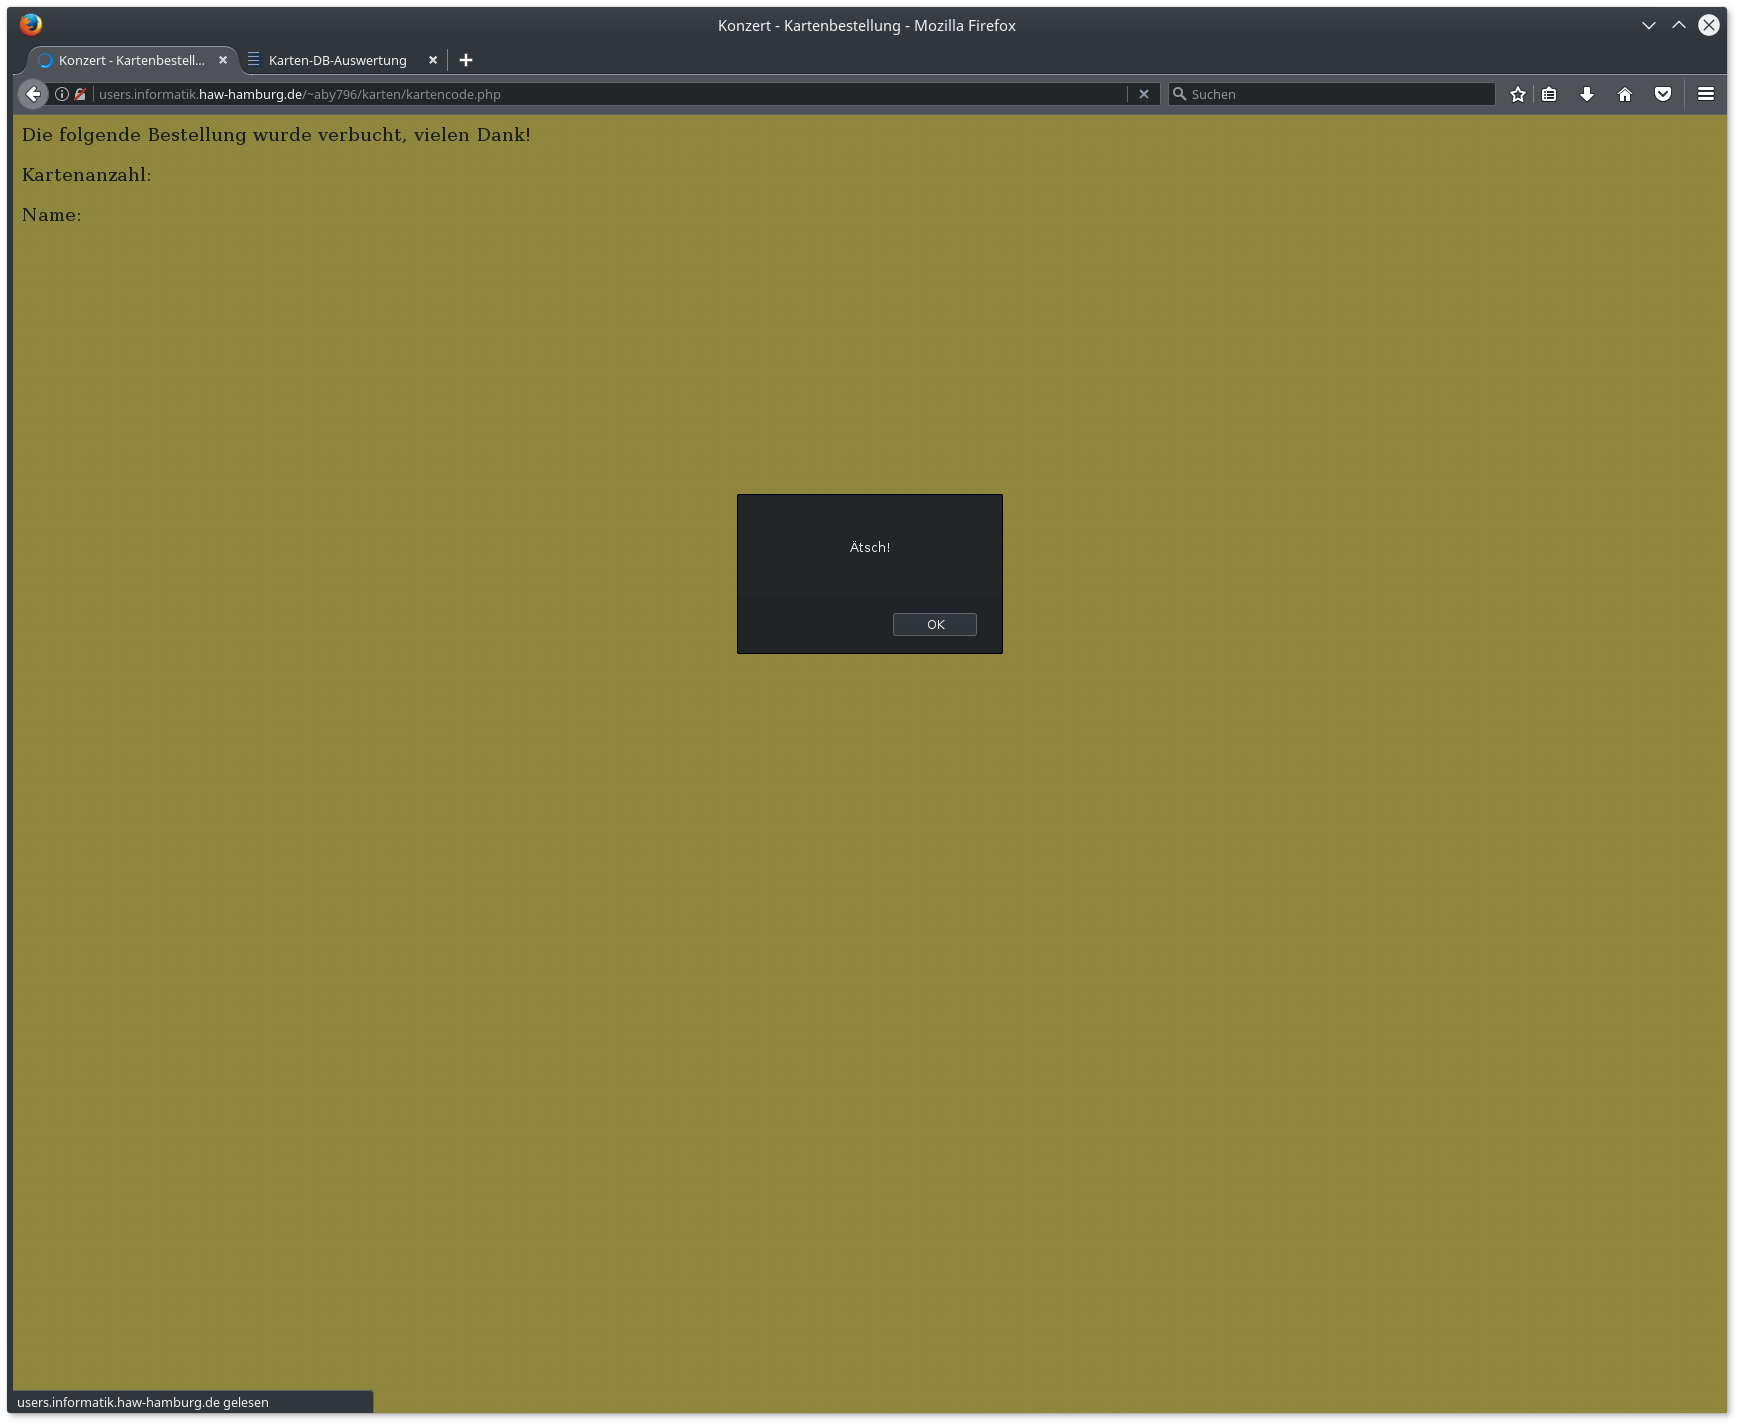
\includegraphics[scale=0.3]{xss.png}
\subsection{XSS - Fix}
XSS-Fix durch Umwandeln von besonderen Zeichen der Eingabe: 
\begin{lstlisting}[language=php]
$Kartenanzahl = htmlspecialchars($_POST['Kartenanzahl'], ENT_QUOTES, 'UTF-8');
$Name = htmlspecialchars($_POST['Name'], ENT_QUOTES, 'UTF-8');
$Strasse = htmlspecialchars($_POST['Strasse'], ENT_QUOTES, 'UTF-8');
$Ort = htmlspecialchars($_POST['Ort'], ENT_QUOTES, 'UTF-8');
$Mail = htmlspecialchars($_POST['Mail'], ENT_QUOTES, 'UTF-8');
\end{lstlisting}
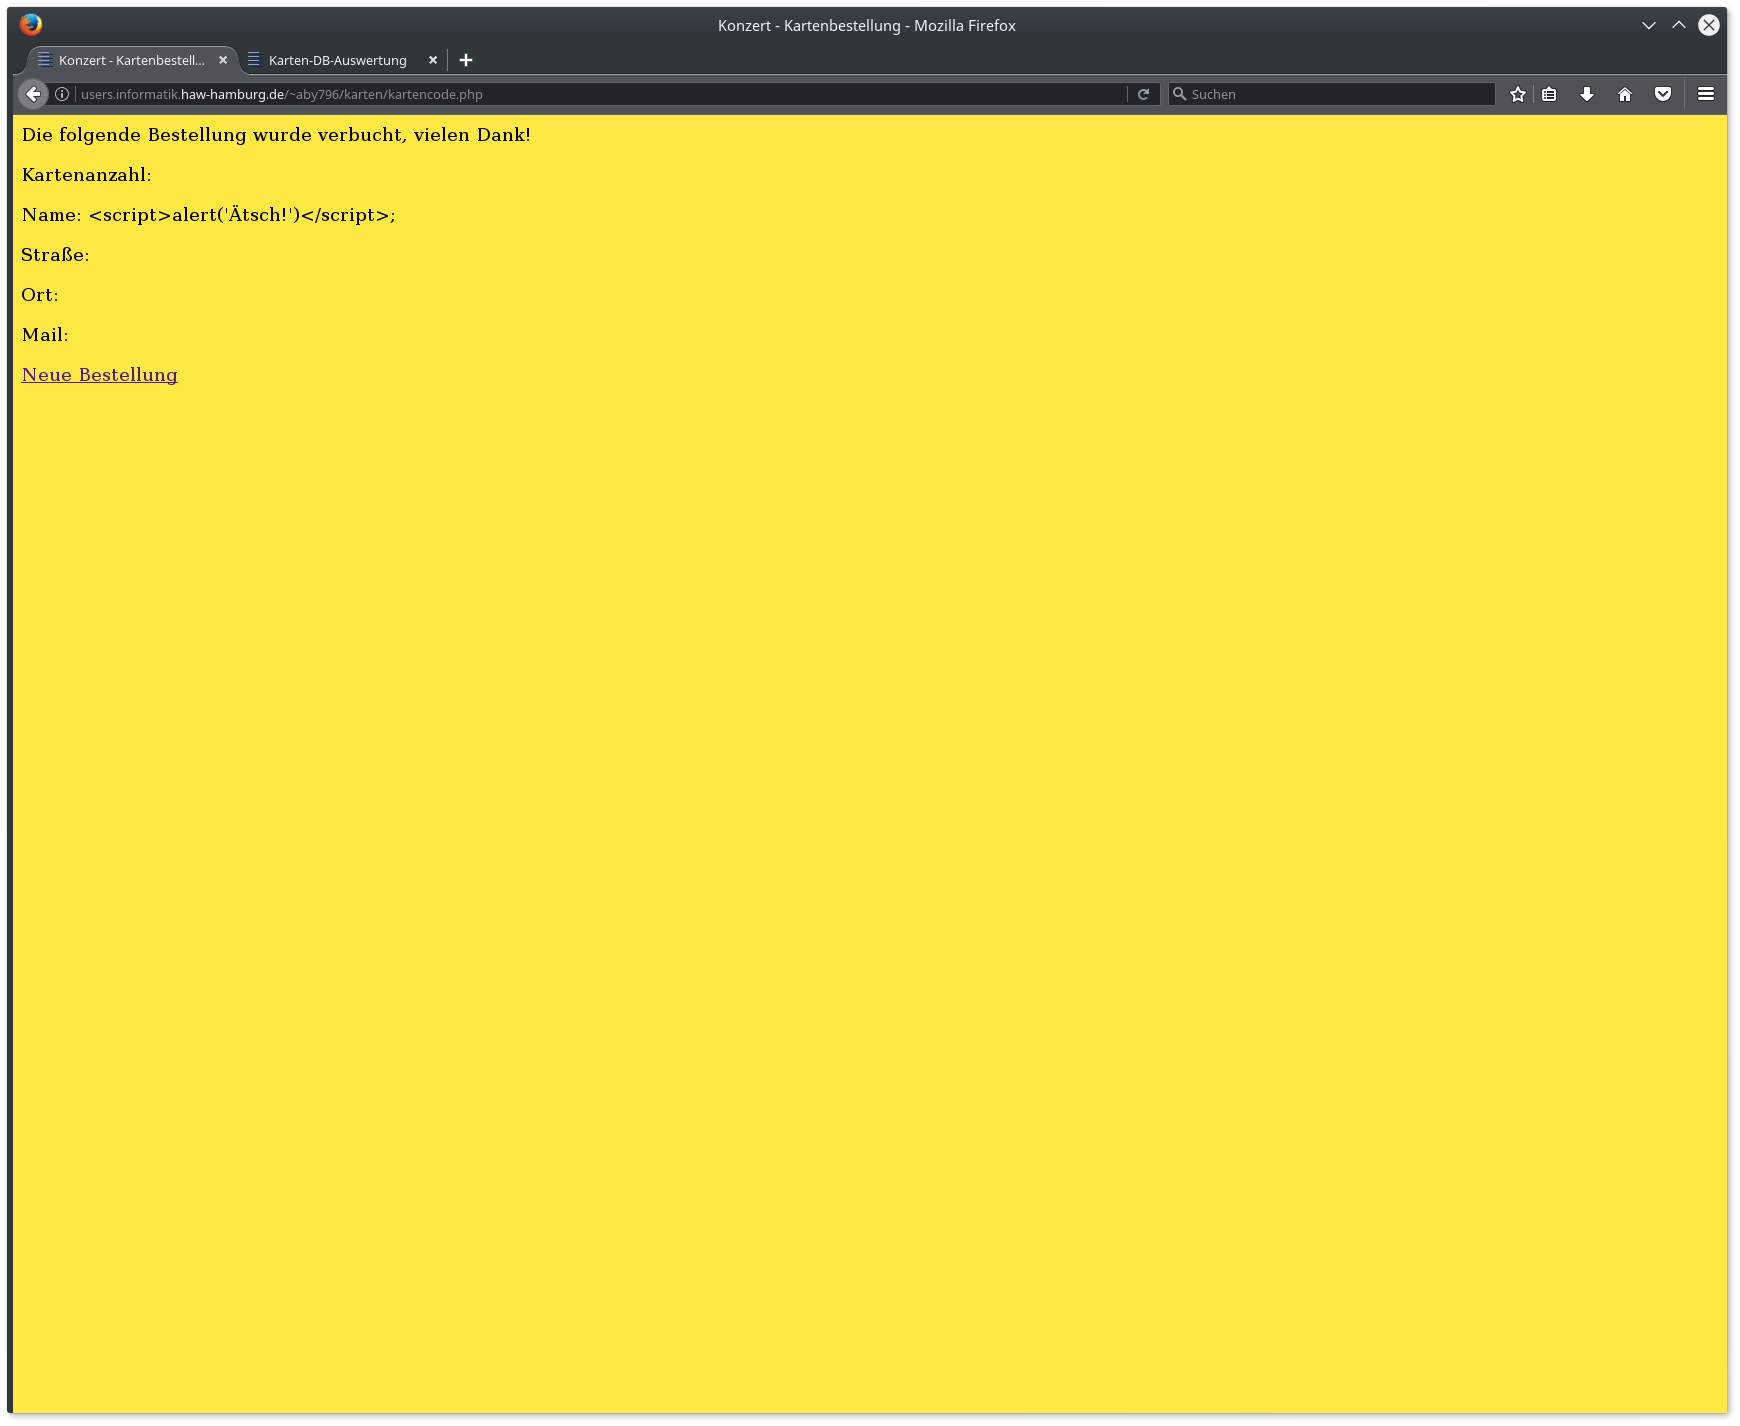
\includegraphics[scale=0.3]{xss_fixed.png}
\subsection{SQL-Injection - Ausführung}
In der Input-Box der Mail-Adresse folgendes Code-Snippet eingeben:
\begin{verbatim}
Test'); DROP TABLE bestellung; --
\end{verbatim}
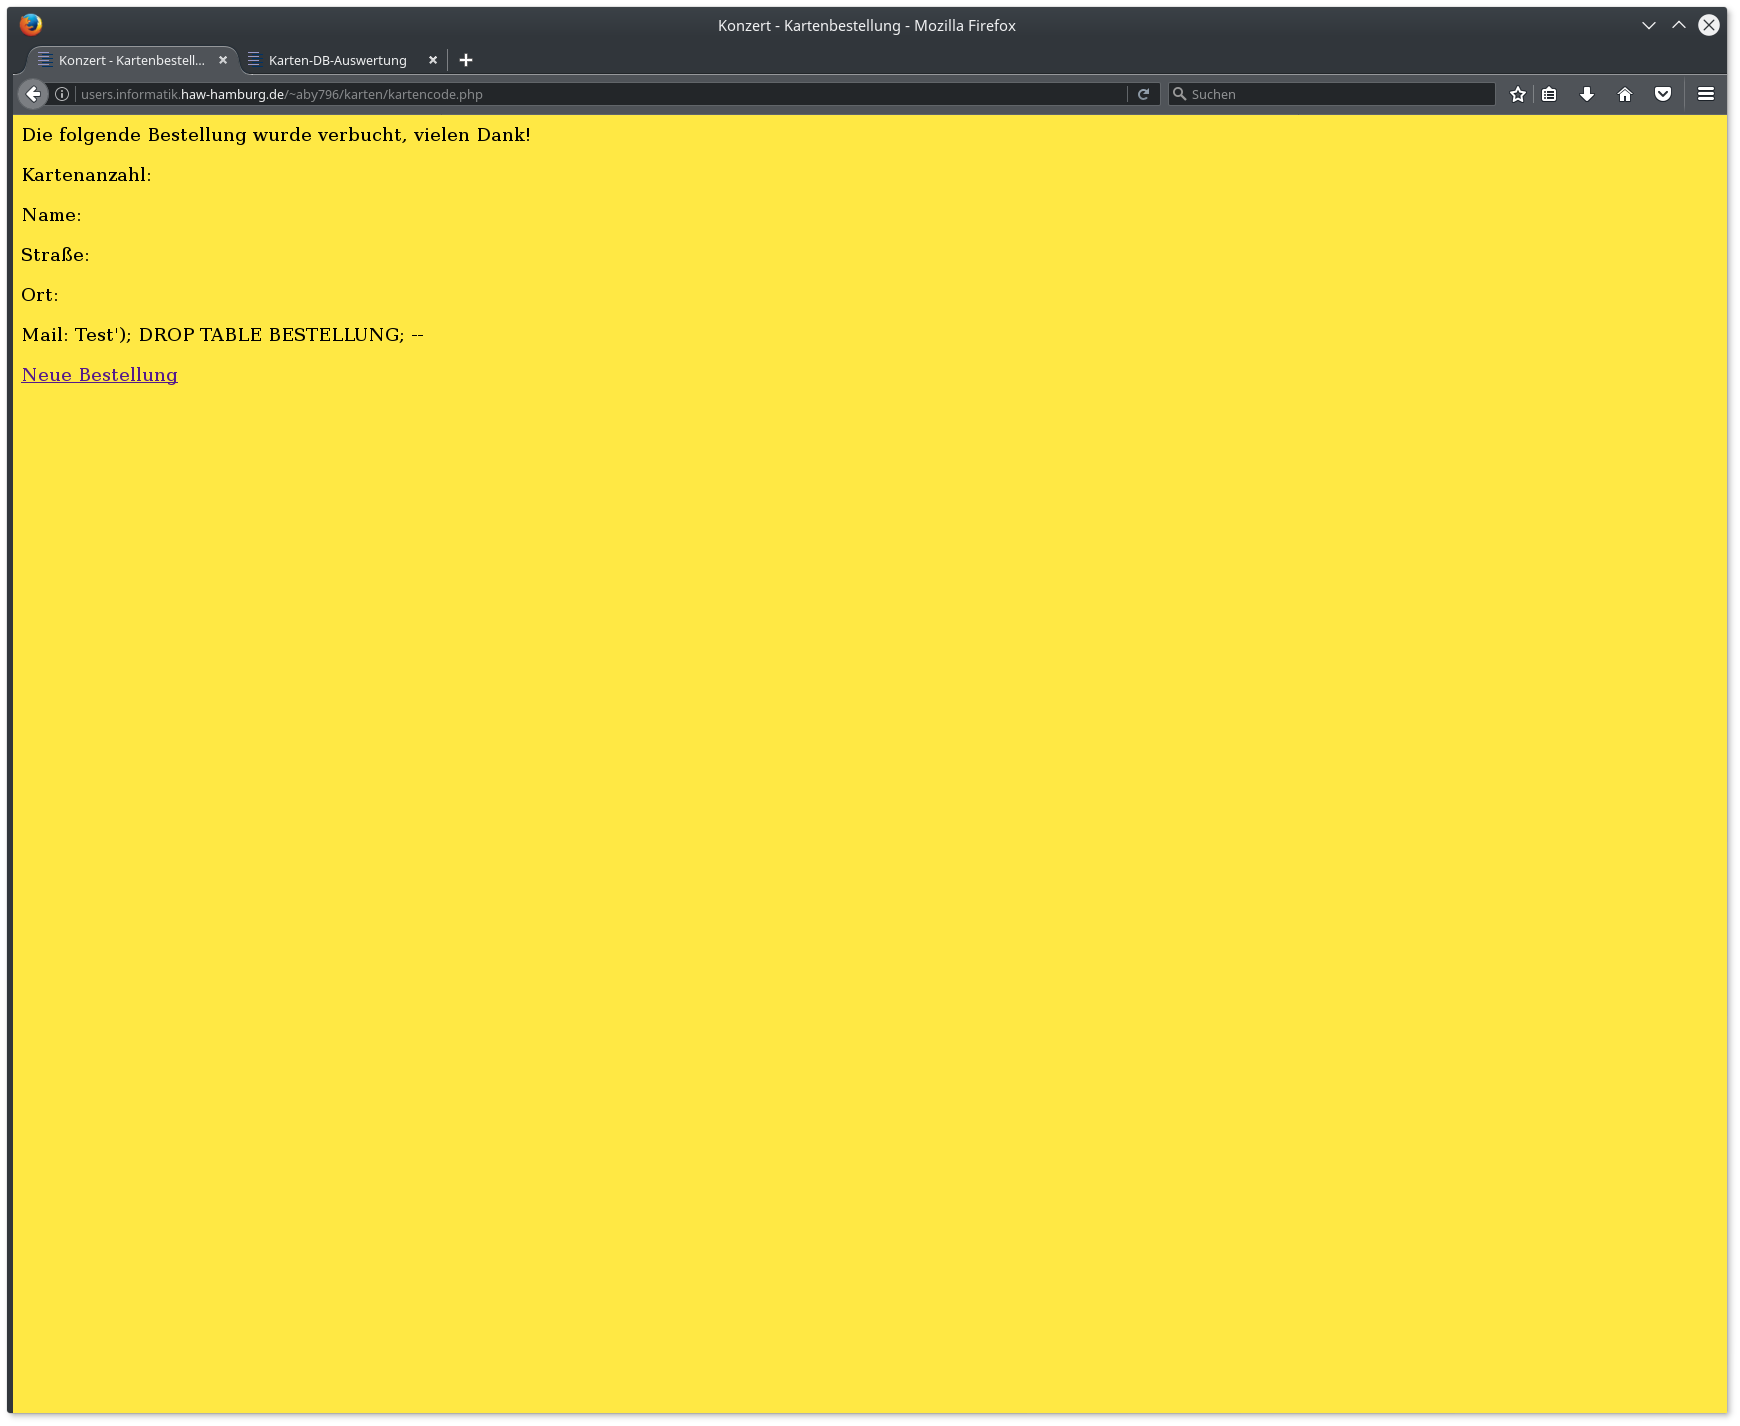
\includegraphics[scale=0.3]{sqli1.png}
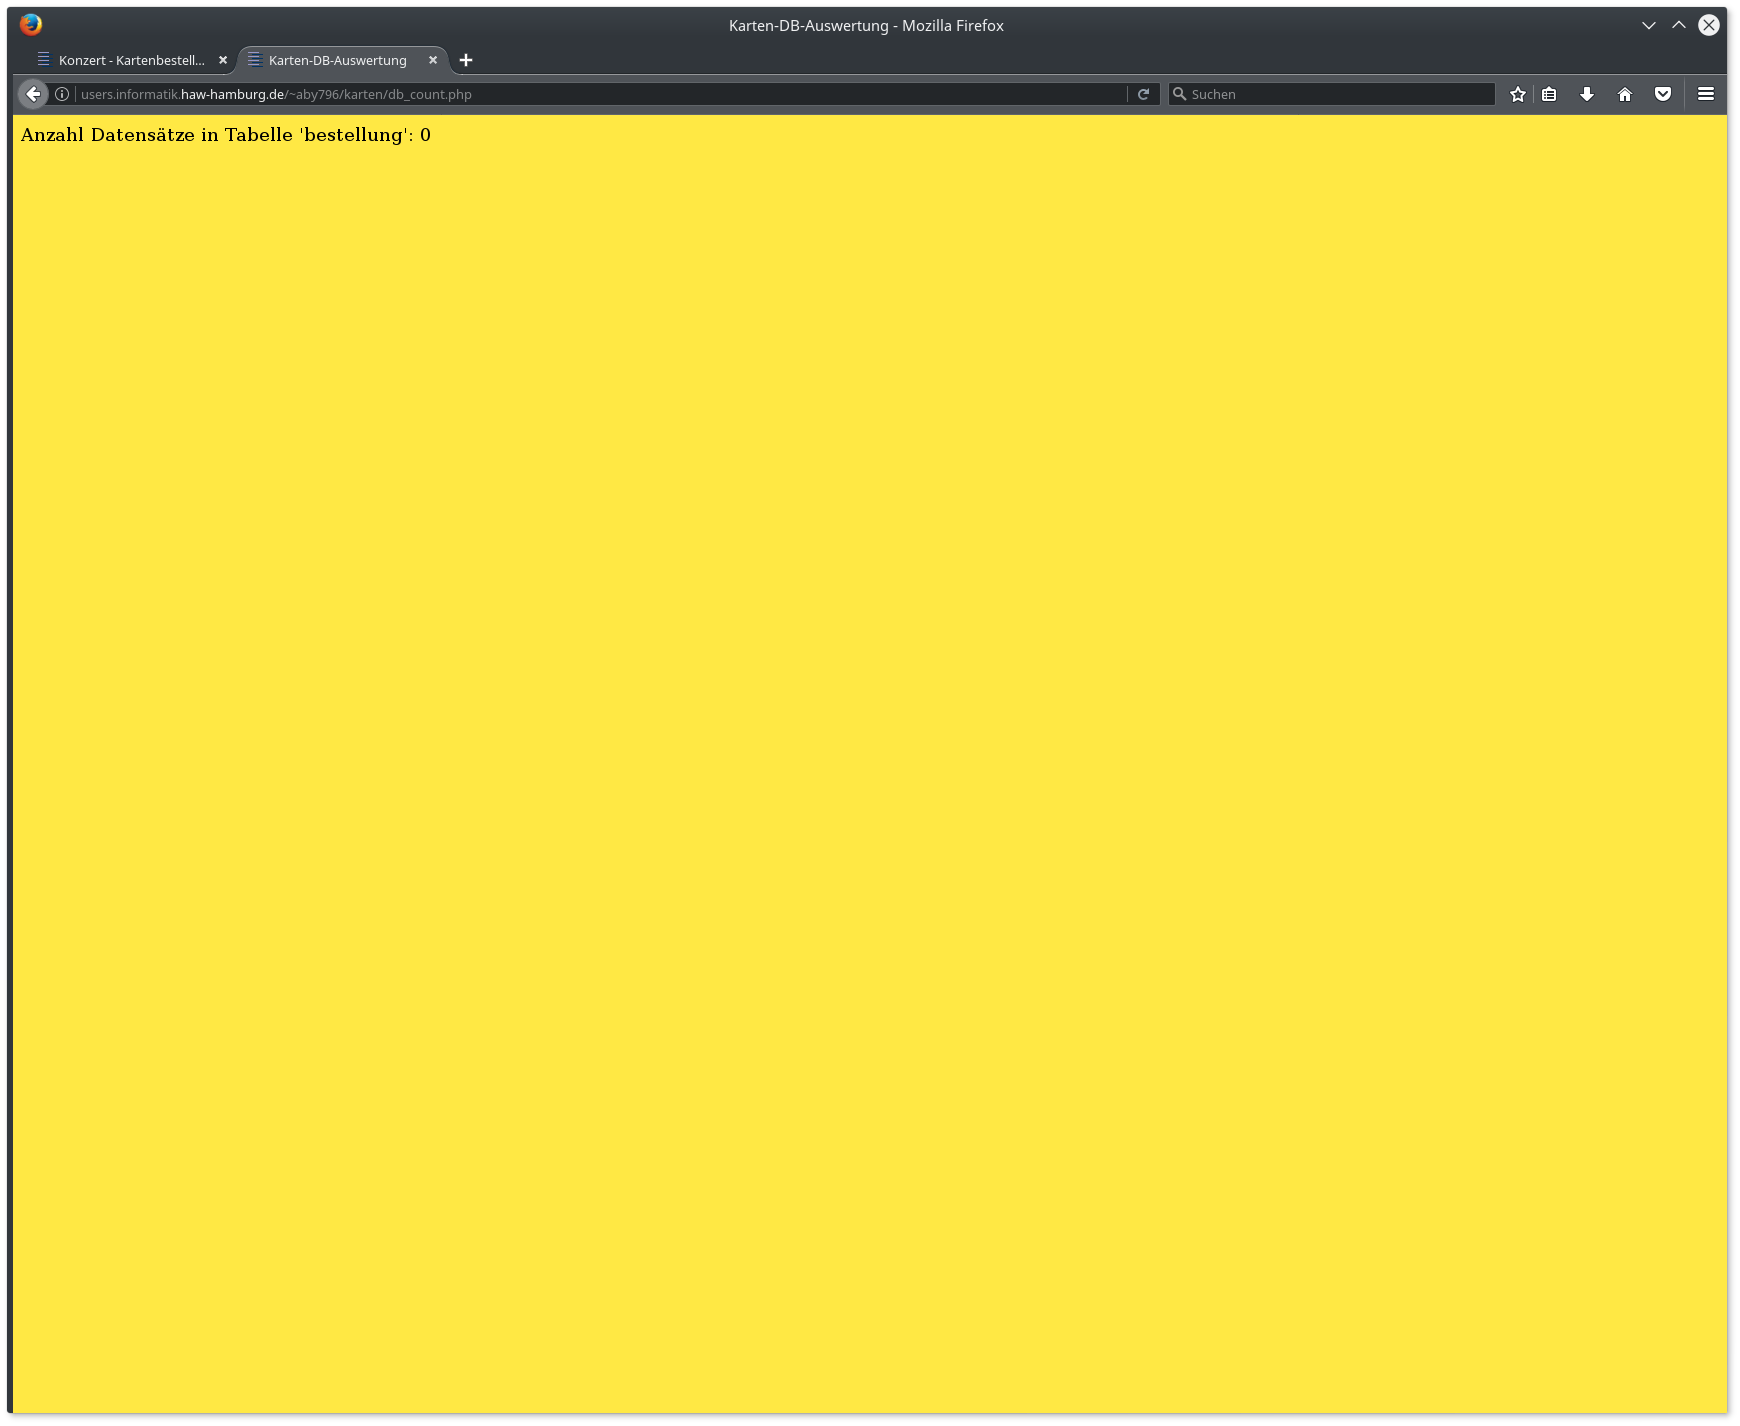
\includegraphics[scale=0.3]{sqli2.png}
\subsection{SQL-Injection - Fix}
SQL-Injection-Fix durch Anwenden eines Prepared-Statements:
\begin{lstlisting}[language=php]
$sql = $db->prepare("INSERT INTO bestellung (anzahl, name, strasse, ort, mail) VALUES (?,?,?,?,?)");
$sql->bindParam(1,$Kartenanzahl);
$sql->bindParam(2,$Name);
$sql->bindParam(3,$Strasse);
$sql->bindParam(4,$Ort);
$sql->bindParam(5,$Mail);

$sql->execute();

\end{lstlisting}

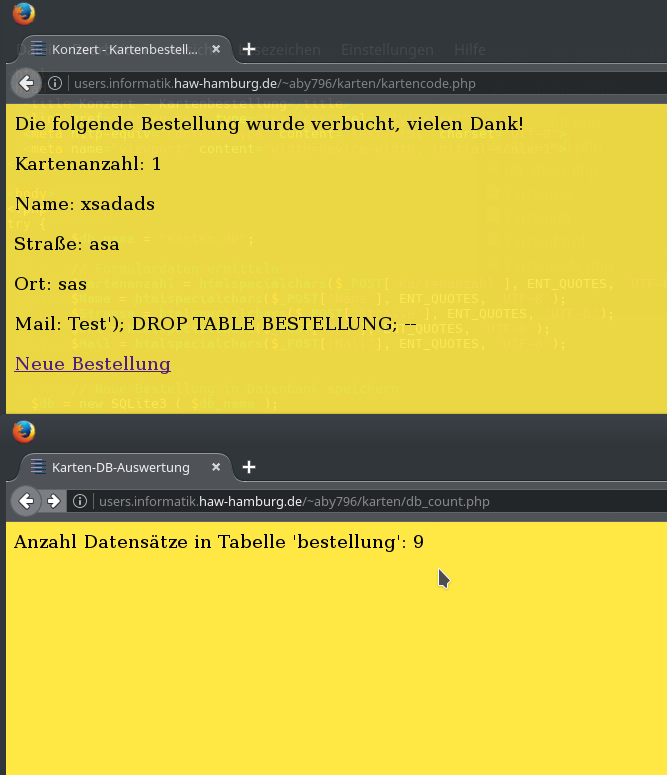
\includegraphics[scale=0.7]{sqli_fixed.png}

\end{document}
